\section{Flaws}
\label{flaws}

% Moved earlier to display nicely in paper
% \flawMnfstsTable{}
% \flawDmnsTable{}

After gathering all these data\footnote{Available in \texttt{ApproachGlossary.csv},
    \texttt{QualityGlossary.csv}, and \texttt{SuppGlossary.csv} at \ifblind{
        [Repository link suppressed]}{
        \url{https://github.com/samm82/TestingTesting}}.}, we find many
flaws. \Cref{fig:flawBars} shows the source tiers (see \Cref{sources})
responsible for these flaws, which reveals a lot about software testing literature:
\begin{enumerate}
    \item Established standards (\Cref{stds}) aren't actually standardized, since:
          \begin{enumerate}
              \item other documents disagree with them \emph{very} frequently and
              \item they are the most internally inconsistent source tier!
          \end{enumerate}
    \item Less standardized (or ``credible''; see \Cref{cred}) documents,
          such as terminology collections and textbooks (\Cref{metas,texts},
          respectively) are also not followed to the extent they should be.
    \item Documents across the board have flaws within the same document,
          between documents with the same author(s), or even with reality%
          \qtodo{Is this too strong of a synonym for ``ground truth''?}!
\end{enumerate}

\ifnotpaper
    \afterpage{\begin{figure}[bt!]
\centering
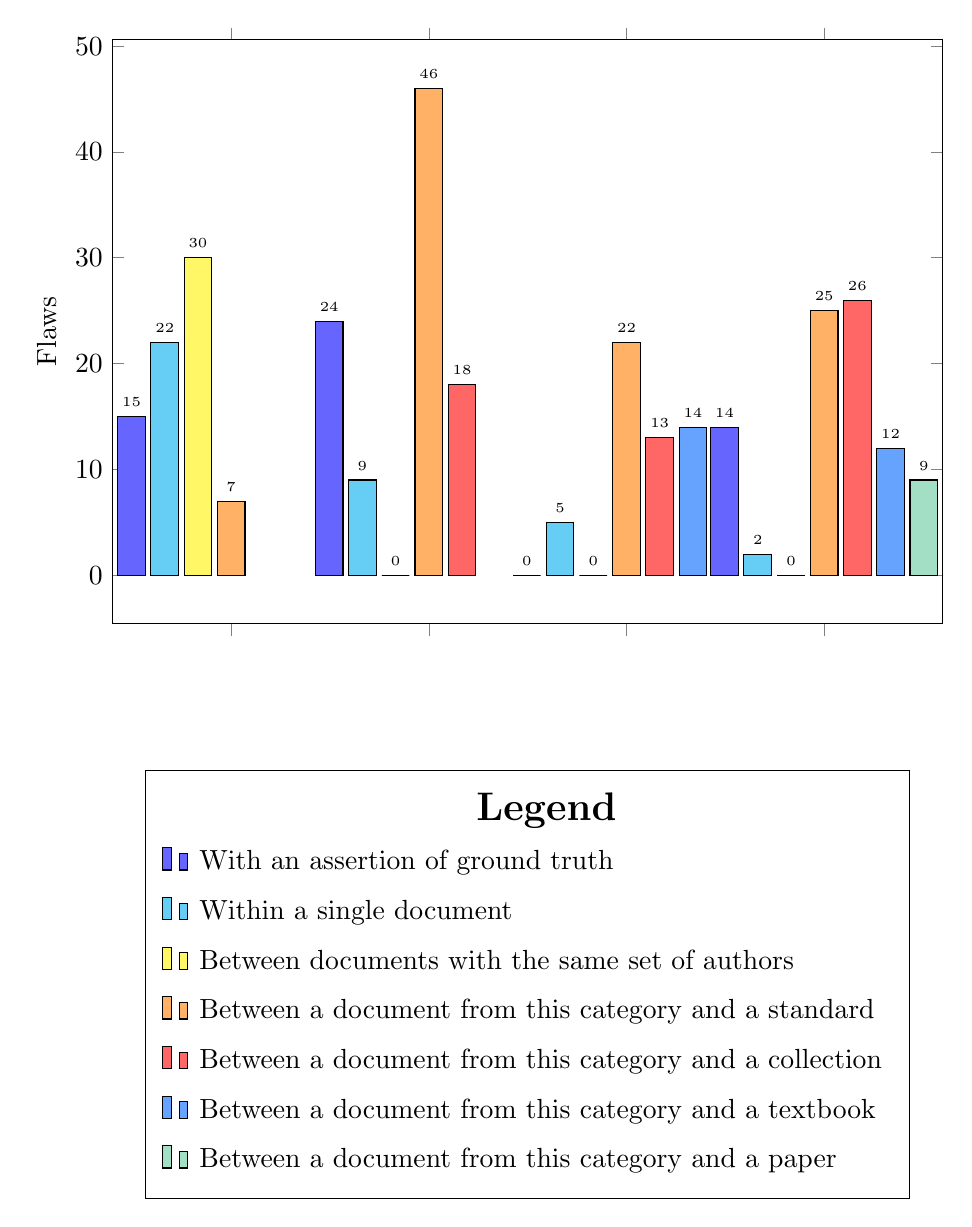
\begin{tikzpicture}
\begin{axis}[
width=\textwidth, height=9cm,
symbolic x coords={std,meta,text,paper},
xtick=data,
xticklabels={{\parbox{0.16\textwidth}{\centering \stds{}}},{\parbox{0.16\textwidth}{\centering \metas{}}},{\parbox{0.16\textwidth}{\centering \texts{}}},{\parbox{0.16\textwidth}{\centering \papers{}}}},
ylabel=Flaws, ybar,
enlargelimits=0.2, enlarge y limits=0.1,
legend style={at={(0.5,-0.25)}, anchor=north, legend columns=1,
inner xsep=6pt,inner ysep=4pt,
nodes={inner sep=4pt,text depth=0.3em},},
legend cell align=left,
nodes near coords,
every node near coord/.append style={font=\tiny},
]
\addlegendimage{empty legend}
\addplot[fill=blue!60] coordinates {(std, 15) (meta, 24) (text, 0) (paper, 14)};
\addplot[fill=cyan!60] coordinates {(std, 22) (meta, 9) (text, 5) (paper, 2)};
\addplot[fill=yellow!60] coordinates {(std, 30) (meta, 0) (text, 0) (paper, 0)};
\addplot[fill=orange!60] coordinates {(std, 7) (meta, 46) (text, 22) (paper, 25)};
\addplot[fill=red!60] coordinates {(meta, 18) (text, 13) (paper, 26)};
\addplot[fill=blue!60!cyan!60] coordinates {(text, 14) (paper, 12)};
\addplot[fill=cyan!60!yellow!60] coordinates {(paper, 9)};
\legend{\hspace{3.4cm} \Large \textbf{Legend},With an assertion of ground truth,Within a single document,Between documents with the same set of authors,Between a document from this category and a standard,Between a document from this category and a collection,Between a document from this category and a textbook,Between a document from this category and a paper}
\end{axis}
\end{tikzpicture}
\caption{Identified flaws by the source tier responsible. Some bars are omitted as they correspond to comparisons we do not make; see \Cref{flaw-cred-compare}.}
\label{fig:flawBars}
\end{figure}
}
    % \begin{figure*}
\centering
\begin{subfigure}[t]{0.475\textwidth}
\begin{tikzpicture}[thick, scale=0.7, every label/.style={align=left, scale=0.7}]
   \pie[text=legend, sum=auto, hide number, color={blue!60, cyan!60, yellow!60, orange!60}]{
      11/15.7\%,
      29/41.4\%,
      25/35.7\%,
      5/7.1\%
}
\end{tikzpicture}
\caption{Flaws found in \stds{}.}
\label{fig:stdFlawSources}
\end{subfigure}
\hfill
\begin{subfigure}[t]{0.475\textwidth}
\begin{tikzpicture}[thick, scale=0.7, every label/.style={align=left, scale=0.7}]
   \pie[text=legend, sum=auto, hide number, color={blue!60, cyan!60, orange!60, red!60}]{
      19/21.1\%,
      10/11.1\%,
      44/48.9\%,
      17/18.9\%
}
\end{tikzpicture}
\caption{Flaws found in \metas{}.}
\label{fig:metaFlawSources}
\end{subfigure}
\vskip\baselineskip
\begin{subfigure}[t]{0.475\textwidth}
\begin{tikzpicture}[thick, scale=0.7, every label/.style={align=left, scale=0.7}]
   \pie[text=legend, sum=auto, hide number, color={cyan!60, orange!60, red!60, blue!60!cyan!60}]{
      4/6.9\%,
      26/44.8\%,
      14/24.1\%,
      14/24.1\%
}
\end{tikzpicture}
\caption{Flaws found in \texts{}.}
\label{fig:textFlawSources}
\end{subfigure}
\hfill
\begin{subfigure}[t]{0.475\textwidth}
\begin{tikzpicture}[thick, scale=0.7, every label/.style={align=left, scale=0.7}]
   \pie[text=legend, sum=auto, hide number, color={blue!60, cyan!60, orange!60, red!60, blue!60!cyan!60, cyan!60!yellow!60}]{
      10/13\%,
      3/3.9\%,
      23/29.9\%,
      24/31.2\%,
      10/13\%,
      7/9.1\%
}
\end{tikzpicture}
\caption{Flaws found in \papers{}.}
\label{fig:paperFlawSources}
\end{subfigure}
\vskip\baselineskip
\begin{center}
\begin{subfigure}[t]{\linewidth}
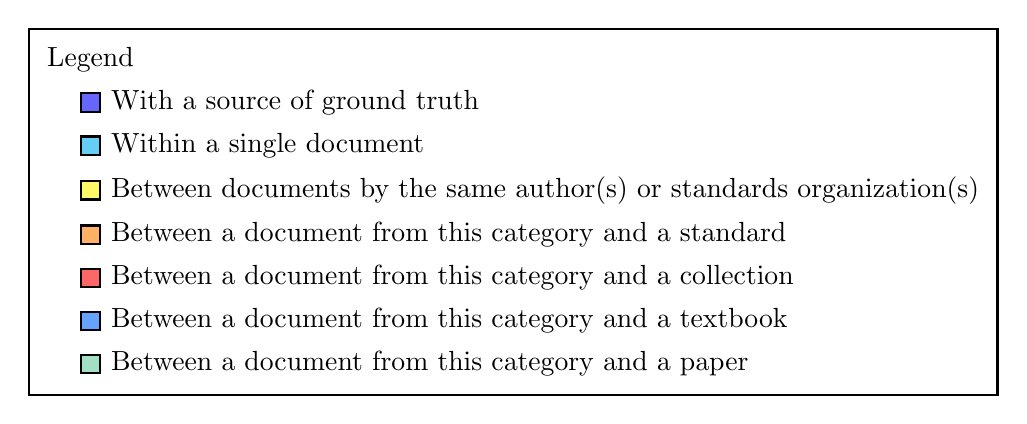
\begin{tikzpicture}
\matrix [thick, draw=black] {
\node[label=center:Legend] {{}}; \\
\node[thick, shape=rectangle, draw=black, fill=blue!60, label=right:{With a source of ground truth}](0) {}; \\
\node[thick, shape=rectangle, draw=black, fill=cyan!60, label=right:{Within a single document}](1) {}; \\
\node[thick, shape=rectangle, draw=black, fill=yellow!60, label=right:{Between documents by the same author(s) or standards organization(s)}](2) {}; \\
\node[thick, shape=rectangle, draw=black, fill=orange!60, label=right:{Between a document from this category and a standard}](3) {}; \\
\node[thick, shape=rectangle, draw=black, fill=red!60, label=right:{Between a document from this category and a collection}](4) {}; \\
\node[thick, shape=rectangle, draw=black, fill=blue!60!cyan!60, label=right:{Between a document from this category and a textbook}](5) {}; \\
\node[thick, shape=rectangle, draw=black, fill=cyan!60!yellow!60, label=right:{Between a document from this category and a paper}](6) {}; \\
};
\end{tikzpicture}
\end{subfigure}
\end{center}
\hfill
\caption{Sources of flaws based on \hyperref[sources]{source tier}.}
\label{fig:flawSources}
\end{figure*}

\fi

To better understand and analyze these flaws, we group them by their
manifestations and their domains as defined in \Cref{flaw-def}.
We present the total number of flaws by manifestation and by domain
in \Cref{tab:flawMnfsts,tab:flawDmns}, respectively, where a given
row corresponds to the number of flaws either within that source tier and/or
with a ``more credible'' one (i.e., a previous row in the table; see
\Cref{cred,sources}). We also group these flaws by their rigidity (defined
in \Cref{rigidity}) by counting (Exp)licit and (Imp)licit flaws separately.
Since we give each flaw a manifestation \emph{and} a domain, the totals per
source and grand totals in these tables are equal. As an example, \tourFlaw*{}.
This is a contradictory definition, so it appears \ifnotpaper as both \else in
\fi \flawref{tour-def-contra,tour-def}. Within these sections, we \ifnotpaper
    list ``more significant'' flaws first, followed by ``less significant''
    ones we omit from the paper version of this thesis. We \else
    omit ``less significant'' flaws for brevity, \fi then sort these flaws
by their source tier (see \Cref{sources}).

We only list flaws we automatically uncover based on their domain \ifnotpaper
    (see \Cref{auto-flaw-analysis}) \fi in their corresponding
domain section for clarity, although they still contribute to the counts in
\Cref{tab:flawMnfsts}. Moreover, certain ``subsets'' of testing contain many
interconnected flaws, which we present in subsections as a ``third view''. This
keeps related information together but causes a further apparent mismatch
between the counts in \Cref{tab:flawMnfsts,tab:flawDmns} and the number of
flaws in \Cref{flawMnfsts,flawDmns}; we still include these flaws in the
manifestation and domain counts\ifnotpaper\ (\Cref{aug-flaw-analysis} outlines
    how this is done)\fi. These subsets include functional testing
(\Cref{func-test-flaw}), \ifnotpaper operational (acceptance) testing
    (\Cref{oat-flaw}), \fi recovery testing (\Cref{recov-flaw}), scalability
testing (\Cref{scal-flaw}), and compatibility testing (\Cref{compat-flaw}).
\ifnotpaper Finally, we infer the more subjective flaws presented in
    \Cref{infer-flaws} which do not contribute to any counts.

    % \input{build/flawTable}

    \begin{landscape}
        \flawMnfstsTable{}
        \flawDmnsTable{}
    \end{landscape}

\fi

\subsection{Flaws by Manifestation}\label{flawMnfsts}

The following sections list observed flaws grouped by \emph{how} they manifest
as presented in \Cref{mnfst-def}. These include mistakes (\Cref{wrong}),
omissions (\Cref{miss}), contradictions (\Cref{contra}), ambiguities
(\Cref{ambi}), \ifnotpaper \else and \fi overlaps (\Cref{over})\ifnotpaper,
and redundancies (\Cref{redun})\fi.

\subsubsection{Mistakes}\label{wrong}
The following are cases where information is incorrect; this includes wrong
definitions (see \Cref{defs}), untrue claims about citations (see \Cref{trace}),
and simple typos:

\input{build/FlawMnfstWrong}

\subsubsection{Omissions}\label{miss}
The following are cases where information (usually definitions; see \Cref{defs})
\emph{should be} included but is not:

\input{build/FlawMnfstMiss}

\subsubsection{Contradictions}\label{contra}
The following are cases where multiple sources of information (sometimes within
the same document!) disagree:

\input{build/FlawMnfstContra}

\subsubsection{Ambiguities}\label{ambi}
The following are cases where information (usually definitions or distinctions
between terms; see \Cref{defs,labels}, respectively) is unclear:

\input{build/FlawMnfstAmbi}

\subsubsection{Overlaps}\label{over}
The following are cases where information overlaps, such as nonatomic
definitions and terms (see \Cref{defs,labels}, respectively):

\input{build/FlawMnfstOver}

\ifnotpaper
    \subsubsection{Redundancies}\label{redun}
    The following are cases of redundant information:

    \input{build/FlawMnfstRedun}
\fi

\subsection{Flaws by Domain}\label{flawDmns}

The following sections list observed flaws grouped by \emph{what} information
is flawed as presented in \Cref{dmn-def}. This includes test approach
categories (\Cref{cats}), synonym relations (\Cref{syns}), parent-child
relations (\Cref{pars}), definitions (\Cref{defs}), labels (\Cref{labels}), and
traceability information (\Cref{trace}).

\subsubsection{Approach Category Flaws}\label{cats}

While the IEEE categorization of testing approaches described in
\Cref{tab:ieeeCats} is useful, it is not without its faults. One issue,
which is not inherent to the categorization itself, is the fact that it is not
used consistently\ifnotpaper\ (see \Cref{tab:otherCats})\fi. The most
blatant example of this is that \ifnotpaper \else ISO/IEC and IEEE \fi
\citet[p.~286]{IEEE2017} describe mutation testing as a
methodology, even though this is not one of the categories \emph{they} created!
Additionally, the boundaries between approaches within a category may
be unclear: ``although each technique is defined independently of all others,
in practice [sic] some can be used in combination with other techniques''
\citep[p.~8]{IEEE2021}. For example, ``the test coverage items derived by
applying equivalence partitioning can be used to identify the input parameters
of test cases derived for scenario testing'' \citetext{p.~8}. Even the categories
themselves are not consistently defined, and some approaches are categorized
differently by different sources; these differences are tracked so
they can be analyzed more systematically\thesisissueref{21}.

\input{build/flawDmnCats}

% Moved here to display nicely in paper
\ifnotpaper\else\begin{paperTable}
    \centering
    \caption{Test approaches with more than one category.}\label{tab:multiCats}
    \begin{minipage}{\linewidth}
        \centering
        \begin{tabular}{|r|l|l|}
            \hline
            \thead{Approach}         & \thead{Category 1}                                                  & \thead{Category 2}                                                                                                                              \\
            \hline
            Ad Hoc Testing           & Practice \cite[p.~33]{IEEE2013}                                     & Technique \cite[p.~5\=/14]{SWEBOK2024}                                                                                                          \\
            Capacity Testing         & Technique \cite[pp.~38\==39]{IEEE2021c}                             & Type \cite[p.~22]{IEEE2022}, \cite[p.~2]{IEEE2013}                                                                                              \\
            Checklist-based Testing  & Practice \cite[p.~34]{IEEE2022}                                     & Technique \cite{ISTQB}                                                                                                                          \\
            Data-driven Testing      & Practice \cite[p.~22]{IEEE2022}                                     & Technique \cite[p.~43]{Kam2008}                                                                                                                 \\
            End-to-end Testing       & Type \cite{ISTQB}                                                   & Technique \cite[p.~47]{Firesmith2015}, \cite[pp.~601, 603, 605\==606]{SharmaEtAl2021}                                                           \\
            Endurance Testing        & Technique \cite[pp.~38\==39]{IEEE2021c}                             & Type \cite[p.~2]{IEEE2013}                                                                                                                      \\
            %                                                                                                                                                   pp.~iii\==iv, 4, 11, 29, 35, 122, 125, 
            Error Guessing           & Practice \cite[p.~33]{IEEE2013}                                     & Technique \cite[pp.~4, 34, Fig.~2]{IEEE2022}, \cite[Fig.~2, Tab.~A.2]{IEEE2021c}\footnote{Some sources omitted for brevity.}                    \\ %, \cite[pp.~3, 33]{IEEE2013}, \cite[p.~5\=/13]{SWEBOK2024}, \cite[p.~50]{Firesmith2015} \\
            Experience-based Testing & Technique \cite[pp.~46, 50]{Firesmith2015}, \cite[Fig.~2]{IEEE2022} & Practice \cite[Fig.~2]{IEEE2022}, \cite[p.~viii]{IEEE2021c}, \cite[pp.~iii, 31, 33]{IEEE2013}                                                   \\
            %                                                                                                                                                                                                   TODO: remove footnote duplication
            Exploratory Testing      & Technique \cite[p.~50]{Firesmith2015}, \cite[p.~5\=/14]{SWEBOK2024} & Practice \cite[pp.~11, 20, 34, Fig.~2]{IEEE2022}, \cite[p.~viii]{IEEE2021c}, \cite[p.~5]{IEEE2021a}\footnote{Some sources omitted for brevity.} \\ %, \cite[pp.~13, 33]{IEEE2013} \\
            Load Testing             & Technique \cite[pp.~38\==39]{IEEE2021c}                             & Type \cite[p.~253]{IEEE2017}, \cite[pp.~5, 20, 22]{IEEE2022}, \cite{ISTQB}                                                                      \\
            Performance Testing      & Technique \cite[pp.~38\==39]{IEEE2021c}                             & Type \cite[pp.~7, 22, 26\==27]{IEEE2022}, \cite[p.~7]{IEEE2021c}, \cite[pp.~2, 8]{IEEE2021a}                                                    \\
            Stress Testing           & Technique \cite[pp.~38\==39]{IEEE2021c}                             & Type \cite[p.~442]{IEEE2017}, \cite[pp.~9, 22]{IEEE2022}                                                                                        \\
            \hline
        \end{tabular}
    \end{minipage}
\end{paperTable}
\fi

\phantomsection{}\label{multiCats}

Some category flaws can be detected automatically, such as test
approaches with more than one category. These are given in \Cref{tab:multiCats}
and include experience-based testing, which is of particular note.
\expBasedCatMain{} These authors say ``experience-based testing practices like
exploratory testing \dots\ are not \dots\ techniques for designing test cases'',
although they ``can use \dots\ test techniques'' \citeyearpar[p.~viii]{IEEE2021},
which they support in \citeyearpar[p.~33]{IEEE2022} along with scripted testing.
This implies that ``experience-based test design techniques'' are used \emph{by}
the practice of experience-based testing which is not \emph{itself} a test
technique (and similarly with scripted testing). If this is the case, it blurs
the line between ``practice'' and ``technique'', which may explain why
experience-based testing is categorized inconsistently in the literature%
\thesisissueref{64}.

\ifnotpaper
    \phantomsection{}\label{classFamilyFlaw}
    However, this might mean that a practice such as experience-based testing
    can be viewed as a ``class of test case design techniques''
    \citep[p.~4]{IEEE2022}. If \emph{this} is the case, then test approaches
    that are a collection of specific subtechniques may be considered
    practices. The following test approaches are each described as a ``class'',
    ``family'', or ``collection'' of techniques by the sources given, which
    seems to support this:
    \begin{itemize}
        \item Combinatorial testing (\citealp[p.~3]{IEEE2022};
              \citeyear[p.~2]{IEEE2021}; \citealp[p.~5-11]{SWEBOK2024})
        \item Data flow testing (\citeyear[p.~3]{IEEE2021};
              implied by \citealp[p.~5-13]{SWEBOK2024})
        \item Performance(-related) testing (\citealp[p.~38]{IEEE2021};
              \perfAsFamily*{})
        \item Security testing \citep[implied by][p.~40]{IEEE2021}
        \item Fault tolerance testing \citep[implied by][p.~4\=/11]{SWEBOK2024}
    \end{itemize}
    Of the above, security testing is an outlier, since it is consistently
    categorized as a test type (\citealp[pp.~9, 22, 26--27]{IEEE2022};
    \citeyear[pp.~7, 40, Tab.~A.1]{IEEE2021}; \citeyear[p.~405]{IEEE2017}%
    \todo{OG 2013}; implied by its quality (\citealp{ISO_IEC2023a};
    \citealp[p.~13-4]{SWEBOK2024}); \citealp[p.~53]{Firesmith2015}) despite
    consisting of ``a number of techniques'' \cite[p.~40]{IEEE2021}, although
    this may be \distinctIEEE{technique} In addition, specification-based
    testing and structure-based testing may also be considered ``families''
    since they are quite broad with many subtechniques and are described as
    ``complementary'' alongside experience-based testing
    \citep[p.~8, Fig.~2]{IEEE2021}.
\fi

Subapproaches of experience-based tesing, such as error guessing and
exploratory testing, are also categorized ambiguously, causing confusion on how
categories and parent-child relations (see \Cref{par-chd-rels}) interact.
\refHelper \citet[p.~34\ifnotpaper, emphasis added\fi]{IEEE2022}
\multiAuthHelper{say} that a previous standard \citeyearpar{IEEE2021}
``describes the experience-based test \emph{design technique} of error
guessing. Other experience-based test \emph{practices} include (but are not
limited to) exploratory testing \dots, tours, attacks, and checklist-based
testing''. This seems to imply that error guessing is both a technique
\emph{and} a practice, which does not make sense if these categories are
orthogonal. \ifnotpaper Similarly, the conflicting categorizations of beta
    testing in \Cref{tab:multiCats} may propagate to its children closed beta
    testing and open beta testing; since this is an inferrence, it is omitted
    from that table and instead included in \Cref{tab:infMultiCats}. \fi These
kinds of inconsistencies between parent and child test approach categorizations
may indicate that categories are not transitive or that more thought must be
given to them.

\ifnotpaper
    \begin{landscape}
        \begin{paperTable}
    \centering
    \caption{Test approaches with more than one category.}\label{tab:multiCats}
    \begin{minipage}{\linewidth}
        \centering
        \begin{tabular}{|r|l|l|}
            \hline
            \thead{Approach}         & \thead{Category 1}                                                  & \thead{Category 2}                                                                                                                              \\
            \hline
            Ad Hoc Testing           & Practice \cite[p.~33]{IEEE2013}                                     & Technique \cite[p.~5\=/14]{SWEBOK2024}                                                                                                          \\
            Capacity Testing         & Technique \cite[pp.~38\==39]{IEEE2021c}                             & Type \cite[p.~22]{IEEE2022}, \cite[p.~2]{IEEE2013}                                                                                              \\
            Checklist-based Testing  & Practice \cite[p.~34]{IEEE2022}                                     & Technique \cite{ISTQB}                                                                                                                          \\
            Data-driven Testing      & Practice \cite[p.~22]{IEEE2022}                                     & Technique \cite[p.~43]{Kam2008}                                                                                                                 \\
            End-to-end Testing       & Type \cite{ISTQB}                                                   & Technique \cite[p.~47]{Firesmith2015}, \cite[pp.~601, 603, 605\==606]{SharmaEtAl2021}                                                           \\
            Endurance Testing        & Technique \cite[pp.~38\==39]{IEEE2021c}                             & Type \cite[p.~2]{IEEE2013}                                                                                                                      \\
            %                                                                                                                                                   pp.~iii\==iv, 4, 11, 29, 35, 122, 125, 
            Error Guessing           & Practice \cite[p.~33]{IEEE2013}                                     & Technique \cite[pp.~4, 34, Fig.~2]{IEEE2022}, \cite[Fig.~2, Tab.~A.2]{IEEE2021c}\footnote{Some sources omitted for brevity.}                    \\ %, \cite[pp.~3, 33]{IEEE2013}, \cite[p.~5\=/13]{SWEBOK2024}, \cite[p.~50]{Firesmith2015} \\
            Experience-based Testing & Technique \cite[pp.~46, 50]{Firesmith2015}, \cite[Fig.~2]{IEEE2022} & Practice \cite[Fig.~2]{IEEE2022}, \cite[p.~viii]{IEEE2021c}, \cite[pp.~iii, 31, 33]{IEEE2013}                                                   \\
            %                                                                                                                                                                                                   TODO: remove footnote duplication
            Exploratory Testing      & Technique \cite[p.~50]{Firesmith2015}, \cite[p.~5\=/14]{SWEBOK2024} & Practice \cite[pp.~11, 20, 34, Fig.~2]{IEEE2022}, \cite[p.~viii]{IEEE2021c}, \cite[p.~5]{IEEE2021a}\footnote{Some sources omitted for brevity.} \\ %, \cite[pp.~13, 33]{IEEE2013} \\
            Load Testing             & Technique \cite[pp.~38\==39]{IEEE2021c}                             & Type \cite[p.~253]{IEEE2017}, \cite[pp.~5, 20, 22]{IEEE2022}, \cite{ISTQB}                                                                      \\
            Performance Testing      & Technique \cite[pp.~38\==39]{IEEE2021c}                             & Type \cite[pp.~7, 22, 26\==27]{IEEE2022}, \cite[p.~7]{IEEE2021c}, \cite[pp.~2, 8]{IEEE2021a}                                                    \\
            Stress Testing           & Technique \cite[pp.~38\==39]{IEEE2021c}                             & Type \cite[p.~442]{IEEE2017}, \cite[pp.~9, 22]{IEEE2022}                                                                                        \\
            \hline
        \end{tabular}
    \end{minipage}
\end{paperTable}

    \end{landscape}
\else % Not yet present in paper
\fi

\subsubsection{Synonym Relation Flaws}\label{syns}

As mentioned in \Cref{syn-rels}, synonyms do not inherently signify a
flaw. Unfortunately, there are many instances of incorrect or ambiguous
synonyms, such as the following:

\input{build/flawDmnSyns}

\phantomsection{}
\label{multiSyns}
There are also cases in which a term is given as a synonym to two (or more)
terms that are not synonyms themselves. Sometimes, these terms
\emph{are} synonyms; for example, \citetISTQB{} \multiAuthHelper{say}
``use case testing'', ``user scenario testing'', and ``scenario testing'' are
all synonyms (although there may be a slight distinction; see
\Cref{tab:parSyns} and \flawref{use-case-scenario}).
% Old explanation based on inconsistent citations from Kam2008/ISTQB
%
% use case testing, user scenario testing,
% and scenario testing are synonyms of each other, as shown in
% \Cref{fig:threeWaySyns}.
% \begin{figure}[hbtp!]
%     \centering
%     \begin{tikzpicture}
%
%         \node[ellipse, draw, align=center] (ust) at (10, 0) {User Scenario\\Testing};
%         \node[ellipse, draw, align=center] (st)  at (0, 0)  {Scenario\\Testing};
%         \node[ellipse, draw, align=center] (uct) at (5, 4)  {Use Case\\Testing};
%
%         \draw[thick] (ust) -- (st)  node [midway, align=center, below]     {\citealpISTQB{}};
%         \draw[thick] (st)  -- (uct) node [midway, align=center, left=12pt] {\citealpISTQB{};\\ \citealp[pp.~47--49]{Kam2008}\\ (see \flawref{use-case-scenario})\\};
%         \draw[thick] (uct) -- (ust) node [midway, align=center, right=4pt] {\citealp[p.~48]{Kam2008}\\};
%
%     \end{tikzpicture}
%     \caption{Visual representation of a three-way synonym relation.}
%     \label{fig:threeWaySyns}
% \end{figure}
However, this does not always make sense. We identify \multiSynCount{}
such cases through automatic analysis of the generated graphs\ifnotpaper,
listed below (test approaches in \emph{italics} are synonyms with each other,
but not with other terms not in italics\todo{Better way to handle/display
    this?})\else. The following three are the most prominent examples\fi:

% Moved here to display nicely in paper
\ifnotpaper\else\begin{paperTable}
    \centering
    \caption{Pairs of test approaches with both \hyperref[par-chd-rels]{parent-child} and \hyperref[syn-rels]{synonym} relations.}
    \label{tab:parSyns}
    \begin{minipage}{\linewidth}
        \centering
        \begin{tabular}{|rcl|l|l|}
            \hline
            \thead{``Child''}        & \thead{$\to$} & \thead{``Parent''}                              & \thead{Parent-Child Source(s)}                                        & \thead{Synonym Source(s)}                                                   \\
            \hline
            All Transitions Testing  & $\to$         & State Transition Testing                        & \citep[p.~19]{IEEE2021}                                               & \citep[p.~15]{Kam2008}                                                      \\
            Co-existence Testing     & $\to$         & Compatibility Testing                           & \cite[p.~3]{IEEE2022}, \cite[Tab.~A.1]{IEEE2021}, \cite{ISO_IEC2023a} & \citep[p.~37]{IEEE2021}                                                     \\
            Fault Tolerance Testing  & $\to$         & Robustness Testing\footnote{\ftrnote{}}         & \citep[p.~56]{Firesmith2015}                                          & \citepISTQB{}                                                               \\
            Functional Testing       & $\to$         & Specification-based Testing\footnote{\specfn{}} & \citep[p.~38]{IEEE2021}                                               & \cite[p.~196]{IEEE2017}, \cite[p.~399]{vanVliet2000}, \cite[p.~44]{Kam2008} \\
            Orthogonal Array Testing & $\to$         & Pairwise Testing                                & \citep[p.~1055]{Mandl1985}                                            & \cite[p.~5-11]{SWEBOK2024}, \cite[p.~473]{Valcheva2013}                     \\
            Path Testing             & $\to$         & Exhaustive Testing                              & \citep[pp.~466-467, 476]{PetersAndPedrycz2000}                        & \citep[p.~421]{vanVliet2000}                                                \\
            Performance Testing      & $\to$         & Performance-related Testing                     & \cite[p.~22]{IEEE2022}, \cite[p.~38]{IEEE2021}                        & \citep[p.~1187]{Moghadam2019}                                               \\
            Static Analysis          & $\to$         & Static Testing                                  & \cite[pp.~9, 17, 25, 28]{IEEE2022}, \cite{ISTQB}                      & \citep[p.~438]{PetersAndPedrycz2000}                                        \\
            % Omitted parent-child sources for static row :\cite[Fig.~4, p.~12]{Gerrard2000a}, \cite[p.~3]{Gerrard2000b}                                     
            Structural Testing       & $\to$         & Structure-based Testing                         & \citep[pp.~105\=/121]{Patton2006}                                     & \cite[p.~9]{IEEE2022}, \cite{ISTQB}, \cite[pp.~443\=/444]{IEEE2017}         \\
            Use Case Testing         & $\to$         & Scenario Testing\footnote{\ucstn{}}             & \cite[p.~20]{IEEE2021}\todo{OG Hass, 2008}                            & \cite{ISTQB}, \cite[pp.~47-49]{Kam2008}                                     \\
            \hline
        \end{tabular}
    \end{minipage}
\end{paperTable}
\fi

\begin{enumerate}
    \item \textbf{Invalid Testing:}
\begin{itemize}
    \item Error Tolerance Testing \cite[p.~45]{Kam2008}
    \item Negative Testing \cite{ISTQB} (implied by \cite[p.~10]{IEEE2021b})
\end{itemize}
\item \textbf{Soak Testing:}
\begin{itemize}
    \item Endurance Testing \cite[p.~39]{IEEE2021b}
    \item Reliability Testing\footnote{Endurance testing is given as a child of
              reliability testing by \cite[p.~55]{Firesmith2015}, although the
              terms are not synonyms.} \cite[Tab.~2]{Gerrard2000a},
          \cite[Tab.~1, p.~26]{Gerrard2000b}
\end{itemize}
\item \textbf{Link Testing:}
\begin{itemize}
    \item Branch Testing (implied by \citealp[p.~24]{IEEE2021b})
    \item Component Integration Testing \citep[p.~45]{Kam2008}
    \item Integration Testing (implied by \citealp[p.~13]{Gerrard2000a})
\end{itemize}
\end{enumerate}

\subsubsection{Parent-Child Relation Flaws}\label{pars}

Parent-child relations (defined in \Cref{par-chd-rels}) are also not immune to
flaws\ifnotpaper, such as the following: \input{build/flawDmnPars} \par \else;
for example, \perfSecParFlaw*{}\fi \phantomsection{}\label{selfPars}%
Additionally, some self-referential definitions imply that a test
approach is a parent of itself. Since these are by nature self-contained within
a given source, these are counted \emph{once} as explicit flaws within
their sources in \Cref{tab:flawMnfsts,tab:flawDmns}. \ifnotpaper We identify
    the following \selfCycleCount{} examples through automatic analysis of our
    generated graphs (see \Cref{selfCycles}):
    \input{build/selfCycles} Interestingly, performance testing is \emph{not}
    described as a subapproach of usability testing by \citep{Gerrard2000a,
        Gerrard2000b}, which would have been more meaningful information to
    capture. \else For example, performance and usability testing are both
    given as subapproaches of themselves \cite[Tab.~2]{Gerrard2000a},
    \cite[Tab.~1]{Gerrard2000b}.\fi

\phantomsection{}\label{parSyns}
There are also pairs of synonyms where one is described as a subapproach
of the other, abusing the meaning of ``synonym'' and causing confusion.
We identify \parSynCount{} of these pairs through automatic analysis of the
generated graphs, \ifnotpaper which are \else with the most prominent \fi
given in \Cref{tab:parSyns}\ifnotpaper\ (additional pairs where a flaw
    is inferred are given in \Cref{infParSyns} for completeness)\fi. Of
particular note is the relation between path testing and exhaustive testing.
While \citet[p.~421]{vanVliet2000} claims that path testing done completely
``is equivalent to exhaustively testing the program''\footnote{The
    contradictory definitions of path testing given in \flawref{path-test}
    add another layer of complexity to this claim.}, this overlooks the effects
of input data \ifnotpaper
    (\citealp[pp.~129--130]{IEEE2021}; \citealp[p.~121]{Patton2006};
    \citealp[p.~467]{PetersAndPedrycz2000})
\else
    \cite[p.~121]{Patton2006}, \cite[p.~129]{IEEE2021},
    \cite[p.~467]{PetersAndPedrycz2000}
\fi and implementation issues \citetext{p.~476} % \citep[p.~476]{PetersAndPedrycz2000}
on the code's behaviour. Exhaustive testing
requires ``all combinations of input values \emph{and} preconditions \dots{}
[to be] tested'' \ifnotpaper (\citealp[p.~4, emphasis added]{IEEE2022};
    similar in \citealpISTQB{}; \citealp[p.~121]{Patton2006})\else
    \cite[p.~4]{IEEE2022} (similar in \citealpISTQB{},
    \cite[p.~121]{Patton2006})\fi.
% Flaw count (WRONG, SYNS): {vanVliet2000} | {IEEE2022} ISTQB {Patton2006}

\ifnotpaper
    \begin{landscape}
        \begin{paperTable}
    \centering
    \caption{Pairs of test approaches with both \hyperref[par-chd-rels]{parent-child} and \hyperref[syn-rels]{synonym} relations.}
    \label{tab:parSyns}
    \begin{minipage}{\linewidth}
        \centering
        \begin{tabular}{|rcl|l|l|}
            \hline
            \thead{``Child''}        & \thead{$\to$} & \thead{``Parent''}                              & \thead{Parent-Child Source(s)}                                        & \thead{Synonym Source(s)}                                                   \\
            \hline
            All Transitions Testing  & $\to$         & State Transition Testing                        & \citep[p.~19]{IEEE2021}                                               & \citep[p.~15]{Kam2008}                                                      \\
            Co-existence Testing     & $\to$         & Compatibility Testing                           & \cite[p.~3]{IEEE2022}, \cite[Tab.~A.1]{IEEE2021}, \cite{ISO_IEC2023a} & \citep[p.~37]{IEEE2021}                                                     \\
            Fault Tolerance Testing  & $\to$         & Robustness Testing\footnote{\ftrnote{}}         & \citep[p.~56]{Firesmith2015}                                          & \citepISTQB{}                                                               \\
            Functional Testing       & $\to$         & Specification-based Testing\footnote{\specfn{}} & \citep[p.~38]{IEEE2021}                                               & \cite[p.~196]{IEEE2017}, \cite[p.~399]{vanVliet2000}, \cite[p.~44]{Kam2008} \\
            Orthogonal Array Testing & $\to$         & Pairwise Testing                                & \citep[p.~1055]{Mandl1985}                                            & \cite[p.~5-11]{SWEBOK2024}, \cite[p.~473]{Valcheva2013}                     \\
            Path Testing             & $\to$         & Exhaustive Testing                              & \citep[pp.~466-467, 476]{PetersAndPedrycz2000}                        & \citep[p.~421]{vanVliet2000}                                                \\
            Performance Testing      & $\to$         & Performance-related Testing                     & \cite[p.~22]{IEEE2022}, \cite[p.~38]{IEEE2021}                        & \citep[p.~1187]{Moghadam2019}                                               \\
            Static Analysis          & $\to$         & Static Testing                                  & \cite[pp.~9, 17, 25, 28]{IEEE2022}, \cite{ISTQB}                      & \citep[p.~438]{PetersAndPedrycz2000}                                        \\
            % Omitted parent-child sources for static row :\cite[Fig.~4, p.~12]{Gerrard2000a}, \cite[p.~3]{Gerrard2000b}                                     
            Structural Testing       & $\to$         & Structure-based Testing                         & \citep[pp.~105\=/121]{Patton2006}                                     & \cite[p.~9]{IEEE2022}, \cite{ISTQB}, \cite[pp.~443\=/444]{IEEE2017}         \\
            Use Case Testing         & $\to$         & Scenario Testing\footnote{\ucstn{}}             & \cite[p.~20]{IEEE2021}\todo{OG Hass, 2008}                            & \cite{ISTQB}, \cite[pp.~47-49]{Kam2008}                                     \\
            \hline
        \end{tabular}
    \end{minipage}
\end{paperTable}

    \end{landscape}
\else % Moved earlier to display nicely in paper
\fi

\subsubsection{Definition Flaws}\label{defs}

Perhaps the most interesting category for those seeking to understand how to
apply a given test approach, there are many flaws with how test
approaches, as well as supporting terms, are defined:

\begin{table}[tb]
    \centering
    \begin{talltblr}[
        % note{a} = {We use \texttt{WRONG} here to avoid clashing with \texttt{MISS}.},
        caption = {Observed flaw domains.},
        label = {tab:flawDmnDefs}
        ]{
        colspec={|Q[c,m]X[l,m]Q[c,m]|},
        column{3} = {font=\ttfamily}, row{1} = {font=\normalfont},
        width = \columnwidth, rowhead = 1
        }
        \hline
        \thead{Subset of Flaws} & \thead{Knowledge Domain}                               & \thead{Key} \\
        \hline
        \cats{}                 & Approach categories, defined in \Cref{cats-def}        & CATS        \\
        \syns{}                 & Synonym relations, defined in \Cref{syn-rels}          & SYNS        \\
        \pars{}                 & Parent-child relations, defined in \Cref{par-chd-rels} & PARS        \\
        \defs{}                 & Definitions given to terms                             & DEFS        \\
        \terms{}                & Labels or names given to terms                         & TERMS       \\
        \cites{}                & Citation information                                   & CITES       \\
        \hline
    \end{talltblr}
\end{table}

% TODO: re-investigate this after going through the rest of ISO/IEC/IEEE 29119
\ifnotpaper
    Also of note: \citep{IEEE2022, IEEE2021}, from the
    ISO/IEC/IEEE 29119 family of standards, mention the following 23 test
    approaches without defining them. This means that out of the 114 test
    approaches they mention, about 20\% have no associated definition!

    However, the previous version of this standard, \citeyearpar{IEEE2013},
    generally explained two, provided references for two, and explicitly defined
    one of these terms, for a total of five definitions that could (should) have
    been included in \citeyearpar{IEEE2022}! These terms have been
    \underline{underlined}\ifnotpaper%
        , \emph{italicized}, and \textbf{bolded}, respectively%
    \fi. Additionally, entries marked with an asterisk* were defined (at least
    partially) in \citeyearpar{IEEE2017}, which would have been available when
    creating this family of standards. These terms bring the total count of terms
    that could (should) have been defined to nine; almost 40\% of undefined test
    approaches could have been defined!

    \begin{itemize}
        \item \underline{Acceptance Testing*}
        \item Alpha Testing*
        \item Beta Testing*
        \item Capture-Replay Driven Testing
        \item Data-driven Testing
        \item Error-based Testing
        \item Factory Acceptance Testing
        \item Fault Injection Testing
        \item Functional Suitability Testing (also mentioned but not defined in
              \citep{IEEE2017})
        \item \underline{Integration Testing}*
        \item Model Verification
        \item Operational Acceptance Testing
        \item Orthogonal Array Testing
        \item Production Verification Testing
        \item Recovery Testing* (Failover/Recovery Testing, Back-up/Recovery
              Testing, \formatPaper{\textbf}{Backup and Recovery Testing*},
              Recovery*; see \Cref{recov-flaw})
        \item Response-Time Testing
        \item \formatPaper{\emph}{Reviews} (ISO/IEC 20246) (Code Reviews*)
        \item Scalability Testing (defined as a synonym of ``capacity
              testing''; see \Cref{scal-flaw})
        \item Statistical Testing
        \item System Integration Testing (System Integration*)
        \item System Testing* (also mentioned but not defined in \citep{IEEE2013})
        \item \formatPaper{\emph}{Unit Testing*}
              (IEEE Std 1008-1987, IEEE Standard for
              Software Unit Testing implicitly listed in the bibliography!)
        \item User Acceptance Testing
    \end{itemize}
\fi

\subsubsection{Label Flaws}\label{labels}

While some flaws exist because the definition of a term is wrong,
others exist because a term's \emph{name} or \emph{label} is wrong!
\defLabelDistinct{}, which we define in \Cref{label-flaw-def}.
We observe the following label flaws:

\input{build/flawDmnLabels}

\subsubsection{Traceability Flaws}\label{trace}

\ifnotpaper
    The following are examples of traceability flaws, as defined in
    \Cref{trace-flaw-def}:
    \input{build/flawDmnTrace}
\else
    Sometimes a document cites another for a piece of information that does not
    appear! For example, \citet[p.~184]{DoğanEtAl2014} \multiAuthHelper{claim}
    that \citet{SakamotoEtAl2013} \multiAuthHelper{define} ``prime path
    coverage'', but it does not.
\fi


\subsection{Functional Testing}
\label{func-test-flaw}

``Functional testing'' is described alongside many other, likely related,
terms. This leads to confusion about what distinguishes these terms, as shown
by the following five:

\subsubsection{Specification-based Testing}
\label{spec-func-test}
This is defined as ``testing in which the principal test basis is the external
inputs and outputs of the test item'' \citep[p.~9]{IEEE2022}. This agrees
with a definition of ``functional testing'': ``testing that
\dots\ focuses solely on the outputs generated in response to
selected inputs and execution conditions'' \citep[p.~196]{IEEE2017}.
\todo{\citet[p.~399]{vanVliet2000} may list these as synonyms; investigate}
Notably, \citet{IEEE2017} lists both as synonyms of
``black-box testing'' \citetext{pp. 431, 196, respectively}, despite them
sometimes being defined separately. For example, the \acf{istqb} defines
``specification-based testing'' as ``testing based on an analysis of the
specification of the component or system'' \ifnotpaper (and gives ``black-box
    testing'' as a synonym) \fi and ``functional testing'' as ``testing
performed to evaluate if a component or system satisfies functional
requirements'' \ifnotpaper (specifying no synonyms) \citepISTQB{};
    % Flaw count (CONTRA, SYNS): {IEEE2022} {IEEE2017} | ISTQB
    the latter references \citet[p.~196]{IEEE2017}
    (``testing conducted to evaluate the compliance of a system or
    component with specified functional requirements'') which
    \emph{has} ``black-box testing'' as a synonym, and mirrors
    \citet[p.~21]{IEEE2022} (testing ``used to check the implementation
    of functional requirements'')\else \cite{ISTQB}\fi. Overall,
specification-based testing \citep[pp.~2-4,~6-9,~22]{IEEE2022} \ifnotpaper and
    black-box testing (\citealp[p.~5-10]{SWEBOK2024};
    \citealp[p.~3]{SouzaEtAl2017})
    % \else \cite[p.~3]{SouzaEtAl2017}, \cite[p.~5-10]{SWEBOK2024}
    are test design techniques \else is a test design technique \fi used to
``derive corresponding test cases'' \citep[p.~11]{IEEE2022} from
``selected inputs and execution conditions'' \citep[p.~196]{IEEE2017}.

\subsubsection{Correctness Testing}
\label{corr-func-test}
\refHelper \citet[p.~5-7]{SWEBOK2024} says ``test cases can be designed to
check that the functional specifications are correctly implemented, which is
variously referred to in the literature as conformance testing, correctness
testing or functional testing''; this mirrors previous definitions
of ``functional testing'' \ifnotpaper
    (\citealp[p.~21]{IEEE2022}; \citeyear[p.~196]{IEEE2017})
\else
    \cite[p.~21]{IEEE2022}, \cite[p.~196]{IEEE2017}
\fi but groups it with ``correctness
testing''. Since ``correctness'' is a software quality \ifnotpaper
    (\citealp[p.~104]{IEEE2017}; \citealp[p.~3-13]{SWEBOK2024}) \else
    \cite[p.~104]{IEEE2017}, \cite[p.~3-13]{SWEBOK2024} \fi which is
what defines a ``test type'' \citep[p.~15]{IEEE2022}\ifnotpaper\
    (see \Cref{qual-test})\fi,
it seems consistent to label ``functional testing'' as a ``test type''
\ifnotpaper
    \citetext{\citealp[pp.~15,~20,~22]{IEEE2022};
        \citeyear[pp.~7,~38,~Tab.~A.1]{IEEE2021}; \citeyear[p.~4]{IEEE2016}}%
\else
    \cite[pp.~15,~20,~22]{IEEE2022}, \cite[pp.~7,~38,~Tab.~A.1]{IEEE2021},
    \cite[p.~4]{IEEE2016}\fi. However, this conflicts with its categorization
as a ``technique'' if considered a synonym of specification-based testing
(see \Cref{spec-func-test}).
% Flaw count (CONTRA, CATS): {IEEE2022} {IEEE2021} {IEEE2016} implied by {IEEE2017} {SWEBOK2024} {IEEE2022} | {IEEE2022} {SWEBOK2024} {SouzaEtAl2017} {IEEE2017}
Additionally, ``correctness testing'' is listed separately from ``functionality
testing'' by \citet[p.~53]{Firesmith2015}.
% Flaw count (CONTRA, SYNS): {SWEBOK2024} | {Firesmith2015}

\subsubsection{Conformance Testing}
Testing that ensures ``that the functional specifications are correctly
implemented'', and can be called ``conformance testing'' or ``functional
testing'' \citep[p.~5-7]{SWEBOK2024}.
``Conformance testing'' is later defined as testing used ``to
verify that the \acs{sut} conforms to standards, rules,
specifications, requirements, design, processes, or practices''
\citep[p.~5-7]{SWEBOK2024}. This definition seems to be a superset
of testing methods mentioned earlier as the latter includes ``standards,
rules, requirements, design, processes, \dots\ [and]'' practices in
\emph{addition} to specifications!
% Flaw count (OVER, SYNS): {SWEBOK2024} | implied by {SWEBOK2024}

A complicating factor is that ``compliance testing'' is also
(plausibly) given as a synonym of ``conformance testing''
\citep[p.~43]{Kam2008}. However, ``conformance
testing'' can also be defined as testing that evaluates the degree
to which ``results \dots\ fall within the limits that define
acceptable variation for a quality requirement''
\citep[p.~93]{IEEE2017}\todo{OG PMBOK 5th ed.}, which seems to
describe something different.
% Flaw count (AMBI, SYNS): {Kam2008} | implied by {IEEE2017}

% TODO: pull out into Recommendations
% Perhaps this second definition of
% ``conformance testing'' should be used, and the previous definition
% of ``compliance testing'' should be used for describing compliance with
% external standards, rules, etc.~to keep them distinct.

\subsubsection{Functional Suitability Testing}
Procedure testing is
called a ``type of functional suitability testing''
\citep[p.~7]{IEEE2022} but no definition of that term is given.
``Functional suitability'' is the
``capability of a product to provide functions that meet stated and
implied needs of intended users when it is used under specified
conditions'', including meeting ``the functional specification''
\citep{ISO_IEC2023a}. This seems to align with the definition of
``functional testing'' as related to ``black-box/%
specification-based testing''.
\ifnotpaper
    ``Functional suitability'' has
    three child terms: ``functional completeness'' (the ``capability of
    a product to provide a set of functions that covers all the
    specified tasks and intended users' objectives''), ``functional
    correctness'' (the ``capability of a product to provide accurate
    results when used by intended users''), and ``functional
    appropriateness'' (the ``capability of a product to provide
    functions that facilitate the accomplishment of specified tasks and
    objectives'') \citep{ISO_IEC2023a}. Notably, ``functional
    correctness'', which includes precision and accuracy
    (\citealp{ISO_IEC2023a}; \citealpISTQB{}), \else ``Functional
    correctness'', a child of ``functional suitability'', is the ``capability
    of a product to provide accurate results when used by intended users''
    \cite{ISO_IEC2023a} and \fi seems to align with
the quality/ies that would be tested by ``correctness'' testing.

\subsubsection{Functionality Testing}
``Functionality'' is defined as the
``capabilities of the various \dots\ features provided by a product''
\citep[p.~196]{IEEE2017} and is said to be a synonym of
``functional suitability'' \citepISTQB{}, although it seems
like it should really be a synonym of ``functional completeness'' based on
\citep{ISO_IEC2023a}, which would make ``functional suitability'' a
% Flaw count (CONTRA, SYNS): ISTQB | implied by {ISO_IEC2023a}
subapproach. Its associated test type
is implied to be a subapproach of build verification testing
\citepISTQB{} and made distinct from ``functional testing''%
\ifnotpaper; interestingly, security is described as a subapproach of both
non-functional and functionality testing\fi\ \citep[Tab.~2]{Gerrard2000a}.
``Functionality testing'' is listed separately from ``correctness testing'' by
\citet[p.~53]{Firesmith2015}.

\ifnotpaper
    \subsection{Operational (Acceptance) Testing}\label{oat-flaw}
    \paragraph{\texttt{(CONTRA, LABELS)}}
    % Flaw count (CONTRA, LABELS): {IEEE2022} ISTQB | {SWEBOK2024} {ISO_IEC2018} {IEEE2017} {SWEBOK2014}
    There are two names that the literature gives to this test approach:
    \begin{itemize}
        \item \emph{\acf{operat}} (\citealp[p.~22]{IEEE2022};
              \citealpISTQB{}) and
        \item \emph{\acf{ot}} (\citealp{ISO_IEC2018};
              \citealp[p.~303]{IEEE2017}; \citealp[p.~6\=/9, in the context of
                  software engineering operations]{SWEBOK2024};
              \citealp[pp.~4\=/6, 4\=/9]{SWEBOK2014}).
    \end{itemize}

    \paragraph{\texttt{(CONTRA, SYNS)}}
    % Flaw count (CONTRA, SYNS): {Firesmith2015}
    % Ground truth: {LambdaTest2024} {BocchinoAndHamilton1996}
    \refHelper \citet[p.~30]{Firesmith2015} lists the above terms separately,
    but they are considered synonyms elsewhere \citep{LambdaTest2024,
        BocchinoAndHamilton1996}\todo{find more academic sources}; since
    \citeauthor{Firesmith2015} does not define these terms, it is hard to
    evaluate \ifnotpaper his \else its \fi distinction.
\fi

\subsection{Recovery Testing}
\label{recov-flaw}

``Recovery testing'' is ``testing \dots\ aimed at verifying
software restart capabilities after a system crash or other disaster''
\citep[p.~5-9]{SWEBOK2024} including ``recover[ing] the data directly affected
and re-establish[ing] the desired state of the system''
\ifnotpaper
    (\citealp{ISO_IEC2023a}; similar in \citealp[p.~7-10]{SWEBOK2024})
\else
    \cite{ISO_IEC2023a} (similar in \cite[p.~7-10]{SWEBOK2024})
\fi
so that the system ``can perform required functions'' \citep[p.~370]{IEEE2017}.
It is also called ``recoverability testing'' \cite[p.~47]{Kam2008} and
potentially ``restart \& recovery (testing)'' \cite[Fig.~5]{Gerrard2000a}.
% Flaw count (AMBI, SYNS): {Gerrard2000a}
The following terms, along with ``recovery testing'' itself
\citep[p.~22]{IEEE2022} are all classified as test types, and the relations
between them can be found in \Cref{fig:recovery-graph-current}.

%% again, maybe convert to \paragraph ?
\begin{itemize}
    \item \textbf{Recoverability Testing:} Testing ``how well a system or
          software can recover data during an interruption or failure''
          \ifnotpaper
              (\citealp[p.~7-10]{SWEBOK2024}; similar in \citealp{ISO_IEC2023a})
          \else
              \cite[p.~7-10]{SWEBOK2024} (similar in \cite{ISO_IEC2023a})
          \fi
          and ``re-establish the desired state of the system'' \citep{ISO_IEC2023a}.
          Synonym for ``recovery testing'' in \citet[p.~47]{Kam2008}.
    \item \textbf{Disaster/Recovery Testing} serves to evaluate if a system
          can ``return to normal operation after a hardware
          or software failure'' \citep[p.~140]{IEEE2017} or if ``operation of
          the test item can be transferred to a different operating site and
          \dots\ be transferred back again once the failure has been
          resolved'' \citeyearpar[p.~37]{IEEE2021}. These two definitions seem to
          describe different aspects of the system, where the first is
          intrinsic to the hardware/software and the second might not be.
          % Flaw count (OVER, DEFS): {IEEE2017} | {IEEE2021}
    \item \textbf{Backup and Recovery Testing} ``measures the
          degree to which system state can be restored from backup within
          specified parameters of time, cost, completeness, and accuracy in
          the event of failure'' \citep[p.~2]{IEEE2013}. This may be what is
          meant by ``recovery testing'' in the context of performance-related
          testing and seems to correspond to the definition of
          ``disaster/recovery testing'' in \citeyearpar[p.~140]{IEEE2017}.
    \item \textbf{Backup/Recovery Testing:} Testing that determines the
          ability ``to restor[e] from back-up memory in the event of failure,
          without transfer[ing] to a different operating site or back-up
          system'' \citep[p.~37]{IEEE2021}. This seems to correspond to the
          definition of ``disaster/recovery testing'' in
          \citeyearpar[p.~37]{IEEE2021}. It is also given as a subtype of
          ``disaster/recovery testing'', even though that tests if ``operation
          of the test item can be transferred to a different operating site''
          \citetext{p.~37}. % Flaw count (CONTRA, PARS): {IEEE2021} | {IEEE2021}
          It also seems to overlap with ``backup and
          recovery testing'', which adds confusion.
          % Flaw count (OVER, DEFS): {IEEE2021} | {IEEE2013}
    \item \textbf{Failover/Recovery Testing:} Testing that determines the
          ability ``to mov[e] to a back-up system in the event of failure,
          without transfer[ing] to a different operating site''
          \citep[p.~37]{IEEE2021}. This is given as a subtype of
          ``disaster/recovery testing'', even though that tests if ``operation
          of the test item can be transferred to a different operating site''
          \citetext{p.~37}. % Flaw count (CONTRA, PARS): {IEEE2021} | {IEEE2021}
    \item \textbf{Failover Testing:} Testing that ``validates the SUT's
          ability to manage heavy loads or unexpected failure to continue
          typical operations'' \citep[p.~5-9]{SWEBOK2024} by entering a
          ``backup operational mode in which [these responsibilities] \dots\
          are assumed by a secondary system'' \citepISTQB{}. While not
          \emph{explicitly} related to recovery, ``failover/recovery testing''
          also describes the idea of ``failover'', and \citet[p.~56]{Firesmith2015}
          uses the term ``failover and recovery testing'', which could be a
          synonym of both of these terms.
          % Flaw count (AMBI, SYNS): {SWEBOK2024} ISTQB | implied by {Firesmith2015}
\end{itemize}

\subsection{Scalability Testing}\label{scal-flaw}

% There were three ambiguities around the term ``scalability testing'', listed
% below.
The relations between test approaches related to scalability testing
are shown in \Cref{fig:scal-graph-current}.

\paragraph{\texttt{(CONTRA, SYNS)}}

% Flaw count (CONTRA, SYNS): {IEEE2021} | {Firesmith2015} {Bas2024}
\citeauthor{IEEE2021} \citeyearpar[p.~39]{IEEE2021} give
``scalability testing'' as a synonym of ``capacity testing''
while other sources differentiate between the two \ifnotpaper
    (\citealp[p.~53]{Firesmith2015}; \citealp[pp.~22\==23]{Bas2024})%
\else \cite[p.~53]{Firesmith2015}, \cite[pp.~22\==23]{Bas2024}\fi.

\paragraph{\texttt{(CONTRA, DEFS)}}

% Flaw count (CONTRA, DEFS): {IEEE2021} | implied by {ISO_IEC2023a}
\citeauthor{IEEE2021} \citeyearpar[p.~39]{IEEE2021} also include the external
modification of the system as part of ``scalability'' but
\citet{ISO_IEC2023a} \ifnotpaper imply \else implies \fi that it is limited
to the system itself.

\paragraph{\texttt{(WRONG, LABELS)}}

% Flaw count (WRONG, LABELS): {SWEBOK2024}
\citeauthor{SWEBOK2024} \citeyearpar[p.~5\=/9]{SWEBOK2024}'s definition of
``scalability testing'' is really a definition of usability testing!

% \subsection{Performance Testing}
% \label{perf-test-ambiguity}

% Similarly, ``performance'' and ``performance efficiency'' are both given as
% software qualities by \ifnotpaper\citeauthor{IEEE2017}\else
%       \cite[p.~319]{IEEE2017}\fi, with the latter defined as the ``performance
% relative to the amount of resources used under stated conditions''
% \ifnotpaper\citeyearpar[p.~319]{IEEE2017} \fi or the ``capability of a product
% to perform its functions within specified time and throughput parameters and be
% efficient in the use of resources under specified conditions'' \citep{ISO_IEC2023a}.
% Initially, there didn't seem to be any meaningful distinction between the two,
% although the term ``performance testing'' is defined
% \ifnotpaper\citeyearpar[p.~320]{IEEE2017}\else\citetext{p.~320}\fi\
% and used by \ifnotpaper\citeauthor{IEEE2017}\else\cite{IEEE2017}\fi\ and the term
% ``performance efficiency testing'' is \emph{also} used by
% \ifnotpaper\citeauthor{IEEE2017}\else\cite{IEEE2017}\fi\ (but not defined
% explicitly). \ifnotpaper Further discussion\thesisissueref{43} brought us to
%       the conclusion \else It can then be concluded \fi that ``performance
% efficiency testing'' is a subset of ``performance testing'', and the
% difference of ``relative to the amount of resources used'' or ``be efficient in
% the use of resources'' between the two is meaningful.

\subsection{Compatibility Testing}
\label{compat-flaw}

% Flaw count (OVER, DEFS): {IEEE2022} | {IEEE2017} ISTQB {ISO_IEC2023a}
``Compatibility testing'' is defined as ``testing that measures the
degree to which a test item can function satisfactorily alongside
other independent products in a shared environment (co-existence),
and where necessary, exchanges information with other systems or
components (interoperability)'' \citep[p.~3]{IEEE2022}. This
definition is nonatomic as it combines the ideas of ``co-existence''
and ``interoperability''. The term ``interoperability testing'' is
not defined, but is used three times \citep[pp.~22,~43]{IEEE2022}
% Flaw count (WRONG, LABELS): {IEEE2022}
(although the third usage seems like it should be ``portability
testing''). This implies that ``co-existence testing'' and
``interoperability testing'' should be defined as their own terms,
which is supported by definitions of ``co-existence'' and
``interoperability'' often being separate \ifnotpaper
    \citetext{\citealpISTQB{}; \citealp[pp.~73,~237]{IEEE2017}}%
\else
    \cite[pp.~73,~237]{IEEE2017}, \cite{ISTQB}%
\fi, the definition of
``interoperability testing'' from \citet[p.~238]{IEEE2017},
and the decomposition of ``compatibility'' into ``co-existence''
and ``interoperability'' by \citet{ISO_IEC2023a}!
% Flaw count (WRONG, SYNS): implied by {IEEE2021} | {IEEE2022}
The ``interoperability'' element of ``compatibility testing'' is explicitly
excluded by \citet[p.~37]{IEEE2021}, (incorrectly) implying that ``compatibility
testing'' and ``co-existence testing'' are synonyms.
% Flaw count (AMBI, SYNS): {Kam2008} | {IEEE2022}
Furthermore, the definition of ``compatibility testing'' in
\citep[p.~43]{Kam2008} unhelpfully says ``See \emph{interoperability testing}'',
adding another layer of confusion to the direction of their relationship.

\ifnotpaper
    \subsection{Inferred Flaws}
    \label{infer-flaws}
    Along the course of this analysis, we inferred many potential flaws.
    Some of these have a conflicting source while others do not. These are
    excluded from any counts of the numbers of flaws, since they are
    more subjective, but are given below for completeness.

    \subsubsection{Inferred Synonym Flaws}\label{infMultiSyns}
    See \Cref{multiSyns}.

    \begin{enumerate}
        \input{build/infMultiSyns}
    \end{enumerate}

    Additionally, \citet[p.~46]{Kam2008} gives ``program testing'' as a synonym
    of ``component testing'' but it probably should be a synonym of ``system
    testing'' instead.
    % \item \refHelper \citet[p.~46]{Kam2008} gives ``program testing'' as a
    % synonym of ``component testing'' but it probably should be a synonym of
    % ``system testing'' instead.

    \subsubsection{Inferred Parent Flaws}\label{infParSyns}
    As discussed in \Cref{parSyns}, some pairs of synonyms also have a
    parent-child relation, abusing the meaning of ``synonym'' and causing
    confusion. While \Cref{tab:parSyns} gives the cases where both relations
    are supported by the literature, some are less explicit. For example, while
    ``\emph{dynamic testing} is sometimes called \dots{} dynamic analysis''
    (\citealp[p.~438]{PetersAndPedrycz2000}; implied by \citealp[p.~149]{IEEE2017}),
    it could be inferred from their static counterparts that dynamic analysis
    is a \emph{child} of dynamic testing (see
    \citealp[pp.~9, 17, 25, 28]{IEEE2022}; \citealpISTQB{}). Additionally, the
    following automatically generated lists contain examples where at least
    one of these conflicting relations is \emph{not} supported by the
    literature but may, nonetheless, be correct. The relations in the first two
    lists are explicitly given in the literature but may be incorrect, while
    those in the third list are unsubtantiated by the literature and require
    more thought before a recommendation can be made.

    \input{build/infParSyns}

    In addition to this type of flaw, \citep[Tab.~2]{Gerrard2000a} does
    \emph{not} give ``functionality testing'' as a parent of ``end-to-end
    functionality testing''. Finally, \citet[p.~119]{Patton2006} says that
    branch testing is ``the simplest form of path testing'' which is also
    implied by \citet[Fig.~F.1]{IEEE2021}\todo{OG Reid, 1996} and
    \citet[p.~433]{vanVliet2000}. This is true in the example
    \citeauthor{Patton2006} gives, but is not necessarily generalizable; one
    could test the behaviour at branches without testing even a \emph{subset}
    of complete paths, which \citet[p.~316]{IEEE2017} give as a definition of
    ``path testing'' (see \flawref{path-test})!

    \subsubsection{Inferred Category Flaws}
    See \Cref{multiCats}.

    \input{build/infMultiCats}

    \subsubsection{Other Inferred Flaws}
    The following are flaws that, if were more concrete, would also be
    included alongside the other flaws:
    \begin{itemize}
        \item ``Fuzz testing'' is ``tagged'' (?) as ``artificial
              intelligence'' \citep[p.~5]{IEEE2022}.
        \item \citeauthor{Gerrard2000b}'s definition for ``security
              audits'' seems too specific, only applying to ``the products
              installed on a site'' and ``the known vulnerabilities for
              those products'' \citeyearpar[p.~28]{Gerrard2000b}.
    \end{itemize}
\fi